\section{宇宙洪荒}

\subsection{引}
惜余年老而日衰兮,岁忽忽而不反。
登苍天而高举兮,历众山而日远。
观江河之纡曲兮,离四海之沾濡。
攀北极而一息兮,吸沆瀣以充虚。
飞朱鸟使先驱兮,驾太一之象舆。
苍龙蚴虬于左骖兮,白虎骋而为右騑。
建日月以为盖兮,载玉女于后车。
驰骛于杳冥之中兮,休息虖昆仑之墟。
乐穷极而不厌兮,愿从容虖神明。
涉丹水而驼骋兮,右大夏之遗风。
黄鹄之一举兮,知山川之纡曲。
再举兮,睹天地之圜方。
临中国之众人兮,讬回飙乎尚羊。\cite{robinson2025}
乃至少原之野兮,赤松王乔皆在旁。
二子拥瑟而调均兮,余因称乎清商。
澹然而自乐兮,吸众气而翱翔。
念我长生而久仙兮,不如反余之故乡。
黄鹄后时而寄处兮,鸱枭群而制之。
神龙失水而陆居兮,为蝼蚁之所裁。
夫黄鹄神龙犹如此兮,况贤者之逢乱世哉。
寿冉冉而日衰兮,固儃回而不息。
俗流从而不止兮,众枉聚而矫直。
或偷合而苟进兮,或隐居而深藏。
苦称量之不审兮,同权概而就衡。
或推迻而苟容兮,或直言之谔谔。
伤诚是之不察兮,并纫茅丝以为索。
方世俗之幽昏兮,眩白黑之美恶。
放山渊之龟玉兮,相与贵夫砾石。
梅伯数谏而至醢兮,来革顺志而用国。
悲仁人之尽节兮,反为小人之所贼。
比干忠谏而剖心兮,箕子被发而佯狂。
水背流而源竭兮,木去根而不长。
非重躯以虑难兮,惜伤身之无功。如图~\ref{fig:2-1} 所示。
已矣哉!

\begin{customfigure}{梅开二度}
	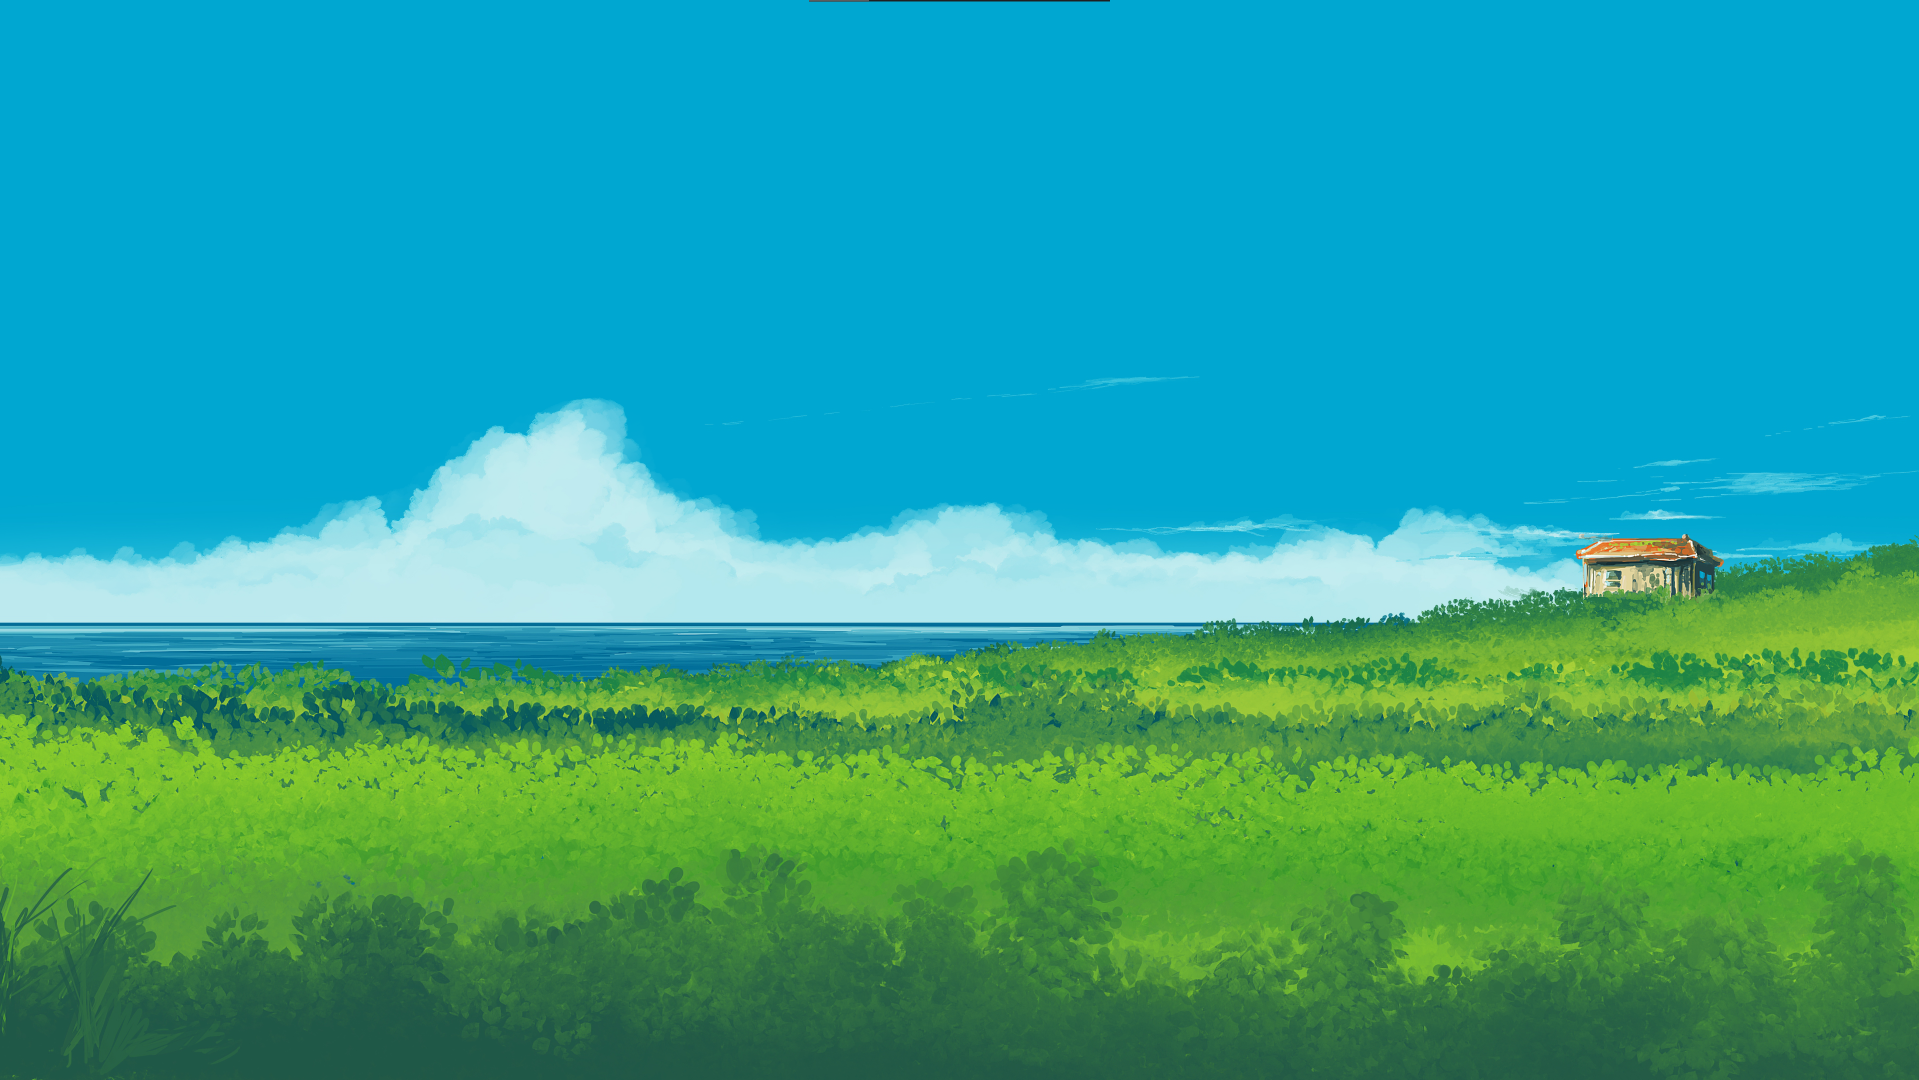
\includegraphics[width=0.8\textwidth]{figures/test2.png} % 你的图片路径
\end{customfigure}

独不见夫鸾凤之高翔兮,乃集大皇之野。
循四极而回周兮,见盛德而后下。
彼圣人之神德兮,远浊世而自藏。
使麒麟可得羁而系兮,又何以异虖犬羊?

\subsection{惜诵}
惜诵以致愍兮,发愤以抒情。
所作忠而言之兮,指苍天以为正。
令五帝使折中兮,戒六神与向服。
俾山川以备御兮,命咎繇使听直。
竭忠诚而事君兮,反离群而赘肬。
忘儇媚以背众兮,待明君其知之。
言与行其可迹兮,情与貌其不变。
故相臣莫若君兮,所以证之不远。
吾谊先君而后身兮,羌众人之所仇也。
专惟君而无他兮,又众兆之所雠也。
壹心而不豫兮,羌无可保也。
疾亲君而无他兮,有招祸之道也。
思君其莫我忠兮,忽忘身之贱贫。
事君而不贰兮,迷不知宠之门。
忠何罪以遇罚兮,亦非余之所志也。
行不群以巅越兮,又众兆之所咍也。如图~\ref{fig:2-2} 所示。
纷逢尤以离谤兮,謇不可释也。

\begin{customfigure}{梅开二度}
	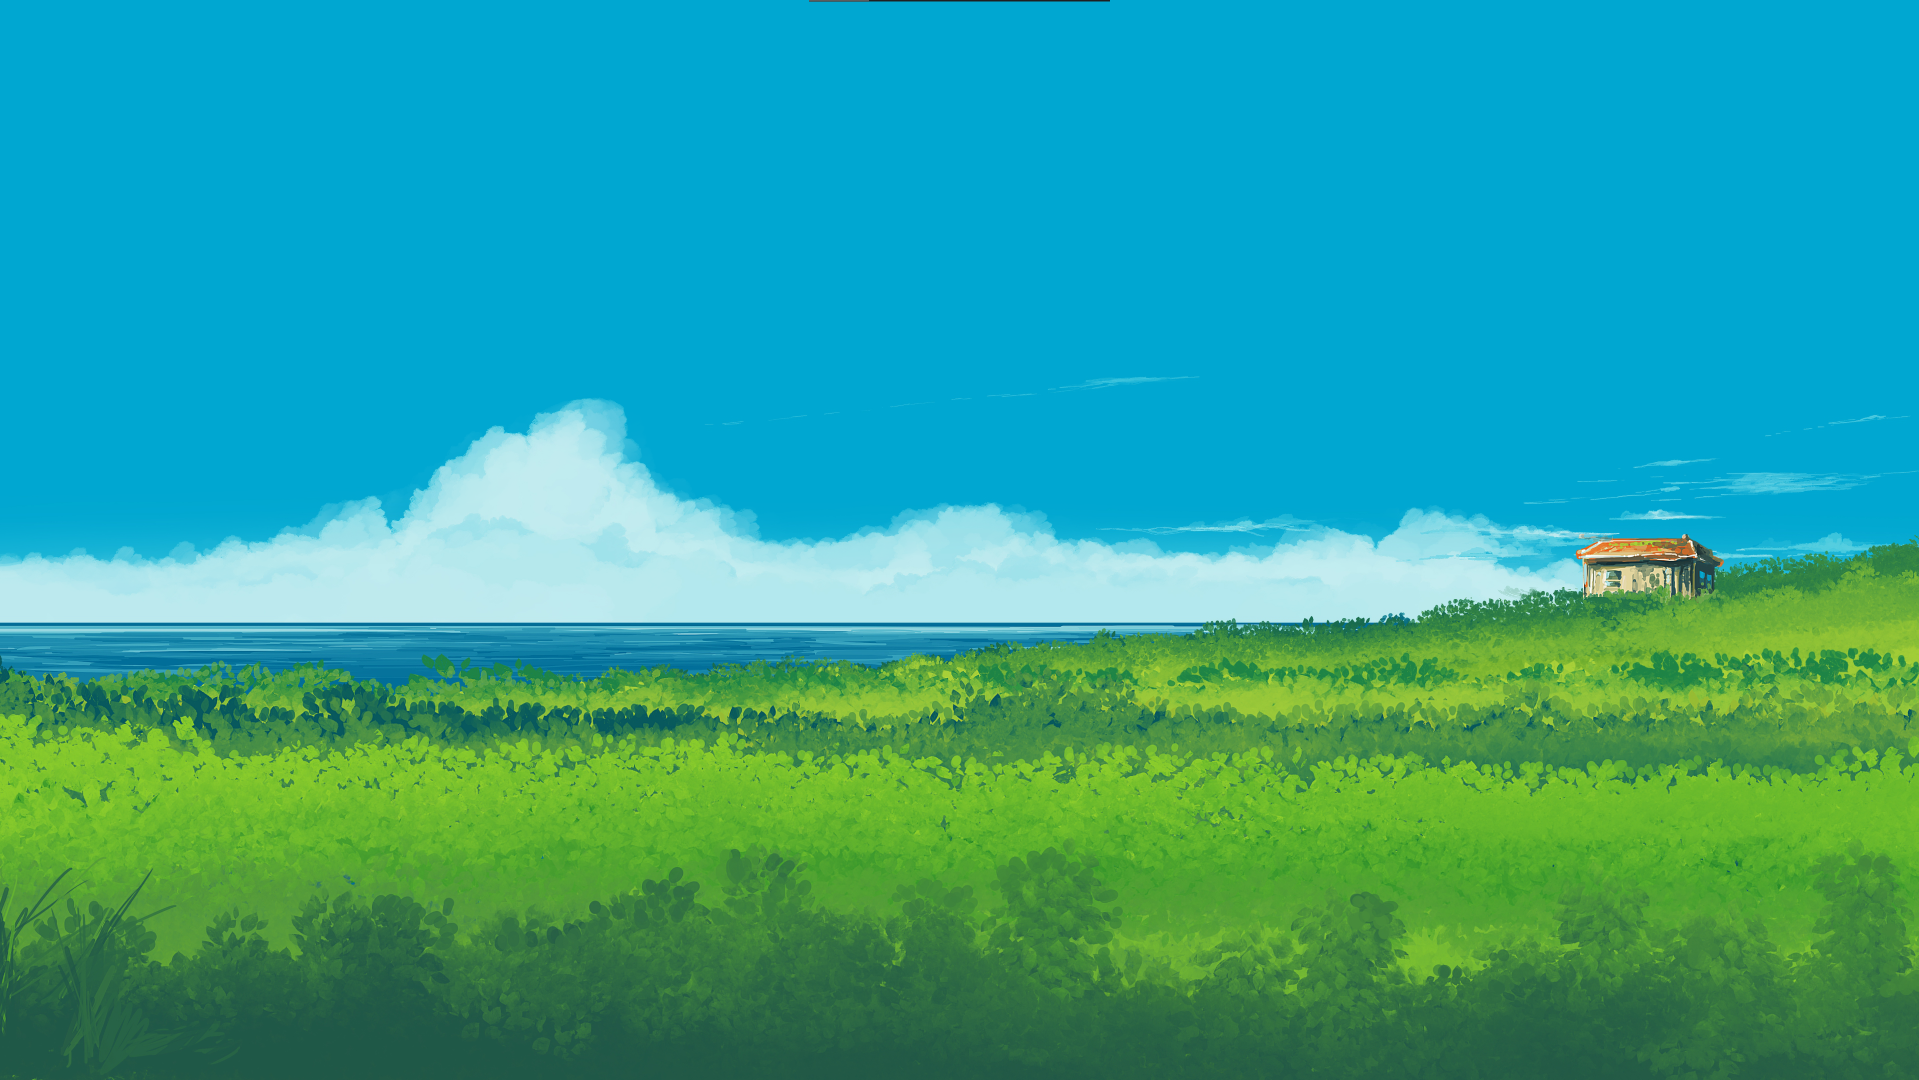
\includegraphics[width=0.8\textwidth]{figures/test2.png} % 你的图片路径
\end{customfigure}

情沉抑而不达兮,又蔽而莫之白也。
心郁邑余侘傺兮,又莫察余之中情。
固烦言不可结而诒兮,愿陈志而无路。
退静默而莫余知兮,进号呼又莫吾闻。
申侘傺之烦惑兮,中闷瞀之忳忳。
昔余梦登天兮,魂中道而无杭。
吾使厉神占之兮,曰有志极而无旁。
终危独以离异兮,曰君可思而不可恃。
故众口其铄金兮,初若是而逢殆。
惩于羹者而吹齑兮,何不变此志也?
欲释阶而登天兮,犹有曩之态也。
众骇遽以离心兮,又何以为此伴也?
同极而异路兮,又何以为此援也?\cite{soares2025,zhang2025,ZhaoYaQi2025}
晋申生之孝子兮,父信谗而不好。
行婞直而不豫兮,鲧功用而不就。
吾闻作忠以造怨兮,忽谓之过言。
九折臂而成医兮,吾至今而知其信然。
矰弋机而在上兮,罻罗张而在下。
设张辟以娱君兮,愿侧身而无所。
欲儃徊以干傺兮,恐重患而离尤。
欲高飞而远集兮,君罔谓汝何之?

\begin{table}[htbp]  % htbp: 这里 (h), 顶部 (t), 底部 (b), 独立页 (p)
	\centering
	\caption{宇宙数据}  % 表题,自动变成黑体,并编号如“表 2.1”
	\label{tab:universe}  % 交叉引用用的 label
	
	\begin{tabular}{ccc}  % 三列表格
		\toprule   % 顶部横线
		星体名称 & 质量 ($M_\odot$) & 距离 (光年) \\  % 表头
		\midrule  % 中部横线
		太阳 & 1.00 & 0 \\
		比邻星 & 0.122 & 4.24 \\
		天狼星 & 2.06 & 8.6 \\
		\bottomrule  % 底部横线
	\end{tabular}
\end{table}


欲横奔而失路兮,盖志坚而不忍。
背膺牉以交痛兮,心郁结而纡轸。如表~\ref{tab:universe} 所示,太阳质量被定义为\begin{math}M_\odot\end{math}。
擣木兰以矫蕙兮,糳申椒以为粮。
播江离与滋菊兮,愿春日以为糗芳。
恐情质之不信兮,故重著以自明。
矫兹媚以私处兮,愿曾思而远身。

\subsection{涉江}
\begin{equation}
	E = mc^2
	\label{eq:example}  % 公式编号
\end{equation}

由公式~\eqref{eq:example} 可得……

余幼好此奇服兮,年既老而不衰。
带长铗之陆离兮,冠切云之崔嵬,
被明月兮佩宝璐。
世混浊而莫余知兮,吾方高驰而不顾。
驾青虬兮骖白螭,吾与重华游兮瑶之圃。
登昆仑兮食玉英,与天地兮同寿,
与日月兮同光。
哀南夷之莫吾知兮,旦余济乎江湘。
乘鄂渚而反顾兮,欸秋冬之绪风。
步余马兮山皋,邸余车兮方林。
乘舲船余上沅兮,齐吴榜以击汰。
船容与而不进兮,淹回水而疑滞。
朝发枉渚兮,夕宿辰阳。
苟余心其端直兮,虽僻远之何伤。
入溆浦余儃徊兮,迷不知吾所如。
深林杳以冥冥兮,乃猿狖之所居。
山峻高以蔽日兮,下幽晦以多雨。
霰雪纷其无垠兮,云霏霏而承宇。
哀吾生之无乐兮,幽独处乎山中。
吾不能变心而从俗兮,固将愁苦而终穷。
接舆髡首兮,桑扈臝行。
忠不必用兮,贤不必以。
伍子逢殃兮,比干菹醢。
与前世而皆然兮,吾又何怨乎今之人!
余将董道而不豫兮,固将重昏而终身!
乱曰:鸾鸟凤皇,日以远兮。
燕雀乌鹊,巢堂坛兮。
露申辛夷,死林薄兮。
腥臊并御,芳不得薄兮。
阴阳易位,时不当兮。
怀信侘傺,忽乎吾将行兮!

\subsection{哀郢}
皇天之不纯命兮,何百姓之震愆?
民离散而相失兮,方仲春而东迁。
去故乡而就远兮,遵江夏以流亡。
出国门而轸怀兮,甲之鼂吾以行。
发郢都而去闾兮,怊荒忽其焉极?
楫齐扬以容与兮,哀见君而不再得。
望长楸而太息兮,涕淫淫其若霰。
过夏首而西浮兮,顾龙门而不见。
心婵媛而伤怀兮,眇不知其所蹠。
顺风波以从流兮,焉洋洋而为客。
凌阳侯之汜滥兮,忽翱翔之焉薄。
心絓结而不解兮,思蹇产而不释。
将运舟而下浮兮,上洞庭而下江。
去终古之所居兮,今逍遥而来东。
羌灵魂之欲归兮,何须臾而忘反。
背夏浦而西思兮,哀故都之日远。
登大坟以远望兮,聊以舒吾忧心。
哀州土之平乐兮,悲江介之遗风。
当陵阳之焉至兮,淼南渡之焉如?
曾不知夏之为丘兮,孰两东门之可芜?
心不怡之长久兮,忧与愁其相接。
惟郢路之辽远兮,江与夏之不可涉。
忽若去不信兮,至今九年而不复。
惨郁郁而不通兮,蹇侘傺而含慼。
外承欢之汋约兮,谌荏弱而难持。
忠湛湛而愿进兮,妒被离而鄣之。
尧舜之抗行兮,瞭杳杳而薄天。
众谗人之嫉妒兮,被以不慈之伪名。
憎愠惀之修美兮,好夫人之慷慨。
众踥蹀而日进兮,美超远而逾迈。
乱曰:
曼余目以流观兮,冀一反之何时?
鸟飞反故乡兮,狐死必首丘。
信非吾罪而弃逐兮,何日夜而忘之?

\subsection{抽思}
心郁郁之忧思兮,独永叹乎增伤。
思蹇产之不释兮,曼遭夜之方长。
悲秋风之动容兮,何回极之浮浮。
数惟荪之多怒兮,伤余心之忧忧。
愿摇起而横奔兮,览民尤以自镇。
结微情以陈词兮,矫以遗夫美人。
昔君与我诚言兮,曰黄昏以为期。
羌中道而回畔兮,反既有此他志。
憍吾以其美好兮,览余以其修姱。
与余言而不信兮,盖为余而造怒。
愿承间而自察兮,心震悼而不敢。
悲夷犹而冀进兮,心怛伤之憺憺。
兹历情以陈辞兮,荪详聋而不闻。
固切人之不媚兮,众果以我为患。
初吾所陈之耿著兮,岂至今其庸亡?
何独乐斯之謇謇兮?愿荪美之可光。
望三王以为像兮,指彭咸以为仪。
夫何极而不至兮,故远闻而难亏。
善不由外来兮,名不可以虚作。
孰无施而有报兮,孰不实而有获?
少歌曰:与美人抽思兮,并日夜而无正。
憍吾以其美好兮,敖朕辞而不听。
倡曰:有鸟自南兮,来集汉北。
好姱佳丽兮,牉独处此异域。
惸茕独而不群兮,又无良媒在其侧。
道卓远而日忘兮,愿自申而不得。
望北山而流涕兮,临流水而太息。
望孟夏之短夜兮,何晦明之若岁?
惟郢路之辽远兮,魂一夕而九逝。
曾不知路之曲直兮,南指月与列星。
愿径逝而未得兮,魂识路之营营。
何灵魂之信直兮,人之心不与吾心同!
理弱而媒不通兮,尚不知余之从容。
乱曰:长濑湍流,溯江潭兮。
狂顾南行,聊以娱心兮。
轸石崴嵬,蹇吾愿兮。
超回志度,行隐进兮。
低徊夷犹,宿北姑兮。
烦冤瞀容,实沛徂兮。
愁叹苦神,灵遥思兮。
路远处幽,又无行媒兮。
道思作颂,聊以自救兮。
忧心不遂,斯言谁告兮。

\subsection{怀沙}
滔滔孟夏兮,草木莽莽。
伤怀永哀兮,汩徂南土。
眴兮杳杳,孔静幽默。
郁结纡轸兮,离慜而长鞠。
抚情效志兮,冤屈而自抑。
刓方以为圜兮,常度未替。
易初本迪兮,君子所鄙。
章画志墨兮,前图未改。
内厚质正兮,大人所盛。
巧倕不斲兮,孰察其拨正。
玄文处幽兮,矇瞍谓之不章;
离娄微睇兮,瞽以为无明。
变白以为黑兮,倒上以为下。
凤皇在笯兮,鸡鹜翔舞。
同糅玉石兮,一概而相量。
夫惟党人之鄙固兮,羌不知余之所臧。
任重载盛兮,陷滞而不济。
怀瑾握瑜兮,穷不知所示。
邑犬之群吠兮,吠所怪也。
非俊疑杰兮,固庸态也。
文质疏内兮,众不知余之异采。
材朴委积兮,莫知余之所有。
重仁袭义兮,谨厚以为丰。
重华不可遌兮,孰知余之从容!
古固有不并兮,岂知其何故也?
汤禹久远兮,邈而不可慕也?
惩违改忿兮,抑心而自强。
离慜而不迁兮,愿志之有像。
进路北次兮,日昧昧其将暮。
舒忧娱哀兮,限之以大故。
乱曰:
浩浩沅湘,分流汩兮。
脩路幽蔽,道远忽兮。
曾唫恒悲兮,永慨叹兮。
世既莫吾知兮,人心不可谓兮。
怀质抱情,独无匹兮。
伯乐既没,骥焉程兮。
民生禀命,各有所错兮。
定心广志,余何畏惧兮!
曾伤爰哀,永叹喟兮。
世浑浊莫吾知,人心不可谓兮。
知死不可让,愿勿爱兮。
明告君子,吾将以为类兮。

